\chapter{IEEE802.15.4g standard }

IoT is a new paradigm in which everyday objects are connected to the Internet. In this evolution of the Internet, conventional objects are granted smart capabilities, allowing them to sense environmental changes, send and receive data and perform tasks. This new network of smart objects opens up a myriad of applications: smart cities, that employ adaptive lighting to optimize energy consumption; smart parking that notifies of available parking spaces; warnings of climate changes; also in healthcare, for remote monitoring of patients and monitor and tracking of vital signs; smart utility networks and smart metering for monitoring of water, oil and gas levels in storage tanks; smart grid for monitoring and management of the electrical system. 

Since the range of applications is very wide, and smart devices are composed of several complex components, major vendors of specific areas are developing their own solutions isolated. Thus, the success of this new technology relies to a large extent on standardization, that will guarantee interoperability, portability, and manageability between devices from different vendors. 

An important feature of the IoT device is its ability to communicate with others devices. The data exchange allows to make decision-based on status, environmental changes etc. Several communications protocols are being used for the IoT, its main features are low-data rates with low power and implementation costs. The following are some of the communications protocols being used in IoT devices:


\begin{itemize}
\item \emph{ZigBee} It is based on the IEEE802.15.4 standard, a standard that defines the operation of LR-WPANs. It specifies the requirements for a low-cost low-power mesh network, it is designed to carry small amounts of data over a short distance while consuming very little power. ZigBee  operates  on the 2.4 Ghz frequency band as well as in the 800-900 sub-GHz bands. 

\item \emph{LoRaWan (Long Range Wide Area Network)}  Developed for long distance networks for national, regional or global areas. Composed mainly of wireless devices powered by batteries. It features bidirectional communications as well as low power consumption, some of the IoT requirements.  

\item \emph{Sigfox}. The basic idea of this technology is to have base stations distributed across some small area and simple devices that can exchange messages with them. A Sigfox message has up to 12-bytes payload and its frame will use 26 bytes in total. It relies on The Ultra Narrow Band modulation technology to exchange messages over the air. Devices requirements are low-power and low-cost. 

\item \emph{WI-SUN}, backed by the Wi-SUN alliance, this technology features low data rates, low power, short-range communication with very low implementation complexity. The Wi-SUN alliance defines the Wireless Smart Ubiquitous Network (Wi-SUN) as a technology
based on the IEEE 802.15.4g standard, an amendment of the IEEE802.15.4 standard. Two profiles are defined by the Wi-SUN Alliance, FAN and HAN networks that support both star and mesh topologies. The communication range is usually from 10 to 75m with low data rate of tens of kbps up to 250 kbps~\cite{sato2015smart}. 

\end{itemize}

%To be able to perform the required tasks, smart objects must be equipped with 
% The Internet of Things is basically a network of interconnected smart objects. In this new kind of network everyday objects will be granted computational and communication capabilities, smart objects will be an integration of several technologies. Thus, expanding its range of application. Based on this concept a myriad of applications appear, smart cities, healthcare, smart homes. The success of this new technology relies on standardization ( Cisco and Forber predicting that the IoT could grow between 50 and 40 billion objects connected by 2020 \cite{forbes}, \cite{cisco}) since it is a growing filed the numbers of solution is rapidly increasing. Standardization will guarantee levels of interoperability, portability and manageability between devices from different vendors. 

%An IoT smart device must be equipped with a processing unit, that process data, sensors and actuators that gathers environmental data and performs specific task. A communication unit that send and receive information from others or to others smart devices. 

%Low power consumption is a must in this smart devices, since they run on batteries most of the time. Thus, hardware and software should be designed to extend battery life to its maximum. 


%SMART GRID     %SMART UTILITY NETWORK = SMART METERING UTILITY NETWORK
%(ELECTRICIDAD) % (SE REFIERE A MEDICION Y COMUNICACION)
%A example of an application for IoT is the Smart Grid. The electrical grid is provided with smart capabilities allowing a two way communication between the customer and the provider. In smart grids smart devices will sense the status of the electrical network, sent data to operation centers and perform managements based on gathered data. Smart metering utility networks (SUNs) enable system control and information transfer in smart grid.  

%Formerly devoted to Smart Metering Utility Network applications and now employed in Smart Ubiquitous Networks (\ac{sunnet}), 

The IEEE 802.15 Working Group for Wireless Specialty Networks developed the 15.4g standard, featuring low-rate wireless connectivity with low power consumption and short-range communication. The IEEE 802.15.4g standard defines Physical (\ac{phy}) and Media Access Control (\ac{mac}) layers requirements for Low-Rate Wireless Personal Area Networks (\ac{LoWPANs}). The next section describes the IEEE802.15.4g standard and some of its features.
%\section{IOT needs standards to be able to live within all the industries that are developing IOT smart devices}

%\subsection{An IOT device has a communication element}

%\subsection{Example of applications Smart Grid}

\section{IEEE802.15.4g Standard}


The IEEE802.15.4g standard is an amendment to the
IEEE802.15.4. It defines alternate PHYs in addition to those in the IEEE802.15.4 as well as modulations,
 data rates, frequency bands and other technical properties. %It enables communication between smart meters and smart grid devices as well as smart home appliances~\cite{anton2014machine}. 

Three PHYs are defined in the IEEE802.15.4g standard:
1) the Multi-rate and 
Multi-Regional Frequency Shift Keying (\ac{fsk}) PHY, with data rates ranging from 50 Kbps to 400 kpbs provides good transmit power efficiency due to the constant envelope of the transmit signal ~\cite{sun_std_2012}, shows low implementation complexity and supports various frequency bands including Europe, Canada, U.S, Korea and Worldwide; 2) The Multi Rate and Multi-Regional Offset Quadrature Phase-Shift Keying  (\ac{qpsk})
PHY shows similar features to those of the IEEE 802.15.4-2011 \ac{qpsk} PHY, thus,  it guarantees interoperability between previously developed devices, it supports Direct Sequence Spread Spectrum (\ac{dsss}) and Multiplexed Direct Sequence Spread Spectrum (\ac{mdsss}). The Multi-Rate and Multi-Regional Orthogonal Frequency Division Multiplexing (\ac{ofdm}) PHY, which provides
 the highest data rates of the three PHYs at the cost of a more complex structure and implementation, it supports data rates ranging from 50 Kpbs to 800 Kbps~\cite{sun_std_2012}. Since the current focus of this work is the development of block concerning the MR-OFDM PHY a more detailed description will be presented in the next section. 
 
\subsection{IEEE802.15.4g MR-OFDM}
\label{sec:mr_ofdm}
%Since the focus of this work is the implementation of blocks concerning the 
%.\ac{ofdm} mode it will be described in detail in this section.



An OFDM modulator can be implemented as an N-point IDFT (see Fig.~\ref{fig:ofdm_tx}), which converts data sequences from frequency domain to time domain, while the demodulator
can be performed by a DFT (see Fig.~\ref{fig:ofdm_rx}) , where each block of N 
received samples is converted back to the frequency domain.
It is well known that the implementation of IDFT/DFT consumes a lot of resources, making mandatory 
the use of the Fast Fourier Transform (\ac{fft}) algorithms, which is one of the addressed topics in this work. 


The MR-OFDM mode as specified in~\cite{sun_std_2012} supports \ac{bpsk}, \ac{qpsk2} and 16-\ac{qam} modulations, depending on the Modulation and Coding Scheme (\ac{mcs}) chosen. Channel encoding is mandatory with a convolutional encoder of coding rate $R =1/2$, it can be punctured to achieve $R = 3/4$. With  \ac{dft} sizes of 128, 64, 32 and 16, the data rates for MR-OFDM ranges from 50 kbps to 800 kbps. Table~\ref{table_mrofdm} shows a summary of the main parameters for the OFDM mode. 

%\begin{table}[htb!]\tiny
\begin{table}[htb!]\footnotesize
\caption{Main Parameters of the MR-OFDM Mode}
\label{table_mrofdm}
\centering
\begin{tabular}{@{}c c c c c c}
\hline
\textbf{PARAMETER}	&\textbf{OPTION 1}	&\textbf{OPTION 2}	&\textbf{OPTION 3}	&\textbf{OPTION 4}	&\textbf{UNIT}\\
\hline\\
SAMPLING RATE		&$1.333\overline{3}$	&$0.666\overline{6}$	&$0.333\overline{3}$ 	&$0.166\overline{6}$	&MSamples/sec\\
FFT SIZE		&$128$			&$64$			&$32$			&$16$			&$\textendash$\\
TONE SPACING		&$10.416\overline{6}$	&$10.416\overline{6}$	&$10.416\overline{6}$	&$10.416\overline{6}$	&KHz\\
FFT DURATION		&$96$			&$96$			&$96$			&$96$			&$\mu s$\\
GI  LENGTH		&$24$			&$24$			&$24$			&$24$			&$\mu s$\\
SYMBOL DURATION		&$120$			&$120$			&$120$			&$120$			&$\mu s$\\
SYMBOL RATE		&$8.333$		&$8.333$		&$8.333$		&$8.333$		&KSymbols/sec\\
ACTIVE TONES		&$104$			&$52$			&$26$			&$14$			&$\textendash$\\
PILOT/DATA/DC TONES	&$8/96/1$		&$4/48/1$		&$2/24/1$		&$2/12/1$		&$\textendash$\\
BANDWIDTH 		&$1094$ 		&$552$			&$281$			&$156$			&KHz\\
%One & Two\\
%\hline
%Three & Four\\
\hline
\end{tabular}
\end{table}

% The MR-OFDM transceiver  contains the 
% transmitter and receiver blocks presented in Fig.~\ref{fig:ofdm_tx} and 
% Fig.~\ref{fig:ofdm_rx}. The main objective of the transmitter is to encode
% the data that will be transmitted and build the PPDU according to the reference
% modulator given by~\cite{sun_std_2012}. Fig.~\ref{fig:ofdm_ppdu_ltf}
% shows the complete \ac{ppdu} structure, which contains: Synchronization Header (\ac{shr}), composed by
% Short Training Field (\ac{stf}) and Long Training Field (\ac{ltf}); PHY Header (\ac{phr}), 
% which carries frame length, scrambling seed, modulation and coding
% scheme (\ac{mcs}); Packet Service Data Unit (\ac{psdu}), which is the PHY payload; PPDU Tail Bits field (TAIL) and Pad Bits (PAD) field.


The \ac{mrofdm} modulator has to encode the data and build the PPDU 
according to the structure defined in~\cite{sun_std_2012}. The PPDU is 
shown in figure~\ref{fig:ofdm_ppdu_ltf}, it contains: Synchronization 
Header (\ac{shr}) used to estimate channel behavior and correct frequency and timing errors. The \ac{shr} is composed by the Short Training Field (\ac{stf}) and Long
Training Field (\ac{ltf}); PHY Header (\ac{phr}), which carries frame 
length, scrambling seed, modulation and coding scheme (\ac{mcs}); Packet
Service Data Unit (\ac{psdu}), the actual payload; PPDU Tail Bits 
field (TAIL) and Pad Bits (PAD) field used to reset and fill buffers. 

\begin{figure}[hbt]
  \centering
    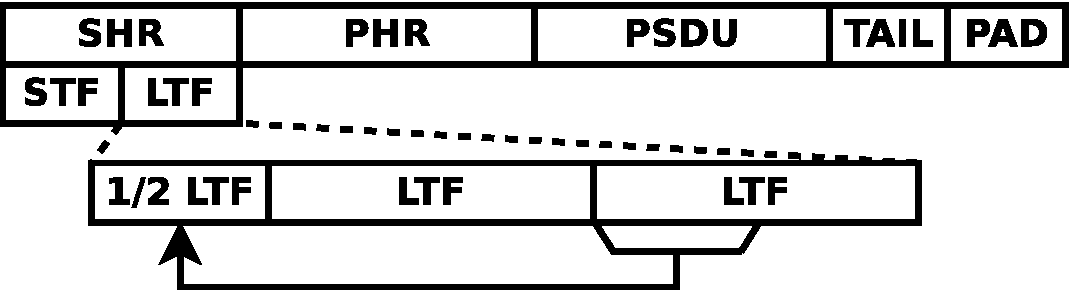
\includegraphics[width=0.6\textwidth]
     {./figuras/ofdm_ppdu_ltf}
%     \rule{35em}{0.5pt}
  \caption{Format of the MR-OFDM PPDU and LTF}
  \label{fig:ofdm_ppdu_ltf}
\end{figure}


The modulator structure is depicted in figure~\ref{fig:ofdm_tx}. This MR-OFDM PHY was designed at Eldorado Research Institute for the ASIC implementation of the IEEE802.15.4g standard, from the reference structure and specification found in \cite{sun_std_2012}. The figure shows the 
modulator divided in data and signal processing. Within the data processing part, conditioning of data bits is performed, it allows error correction and protect the data from channel impairments. From the 
Mapper (point 9 in figure~\ref{fig:ofdm_tx}) onward, digital signal processing is applied, here
signal conditioning is applied to complex decimal data. Referencing figure \ref{fig:ofdm_tx} every numbered point represents  a conditioning or modification of the data, the complete data processing and signal processing is as follows:

\begin{figure}[hbt]
  \centering
    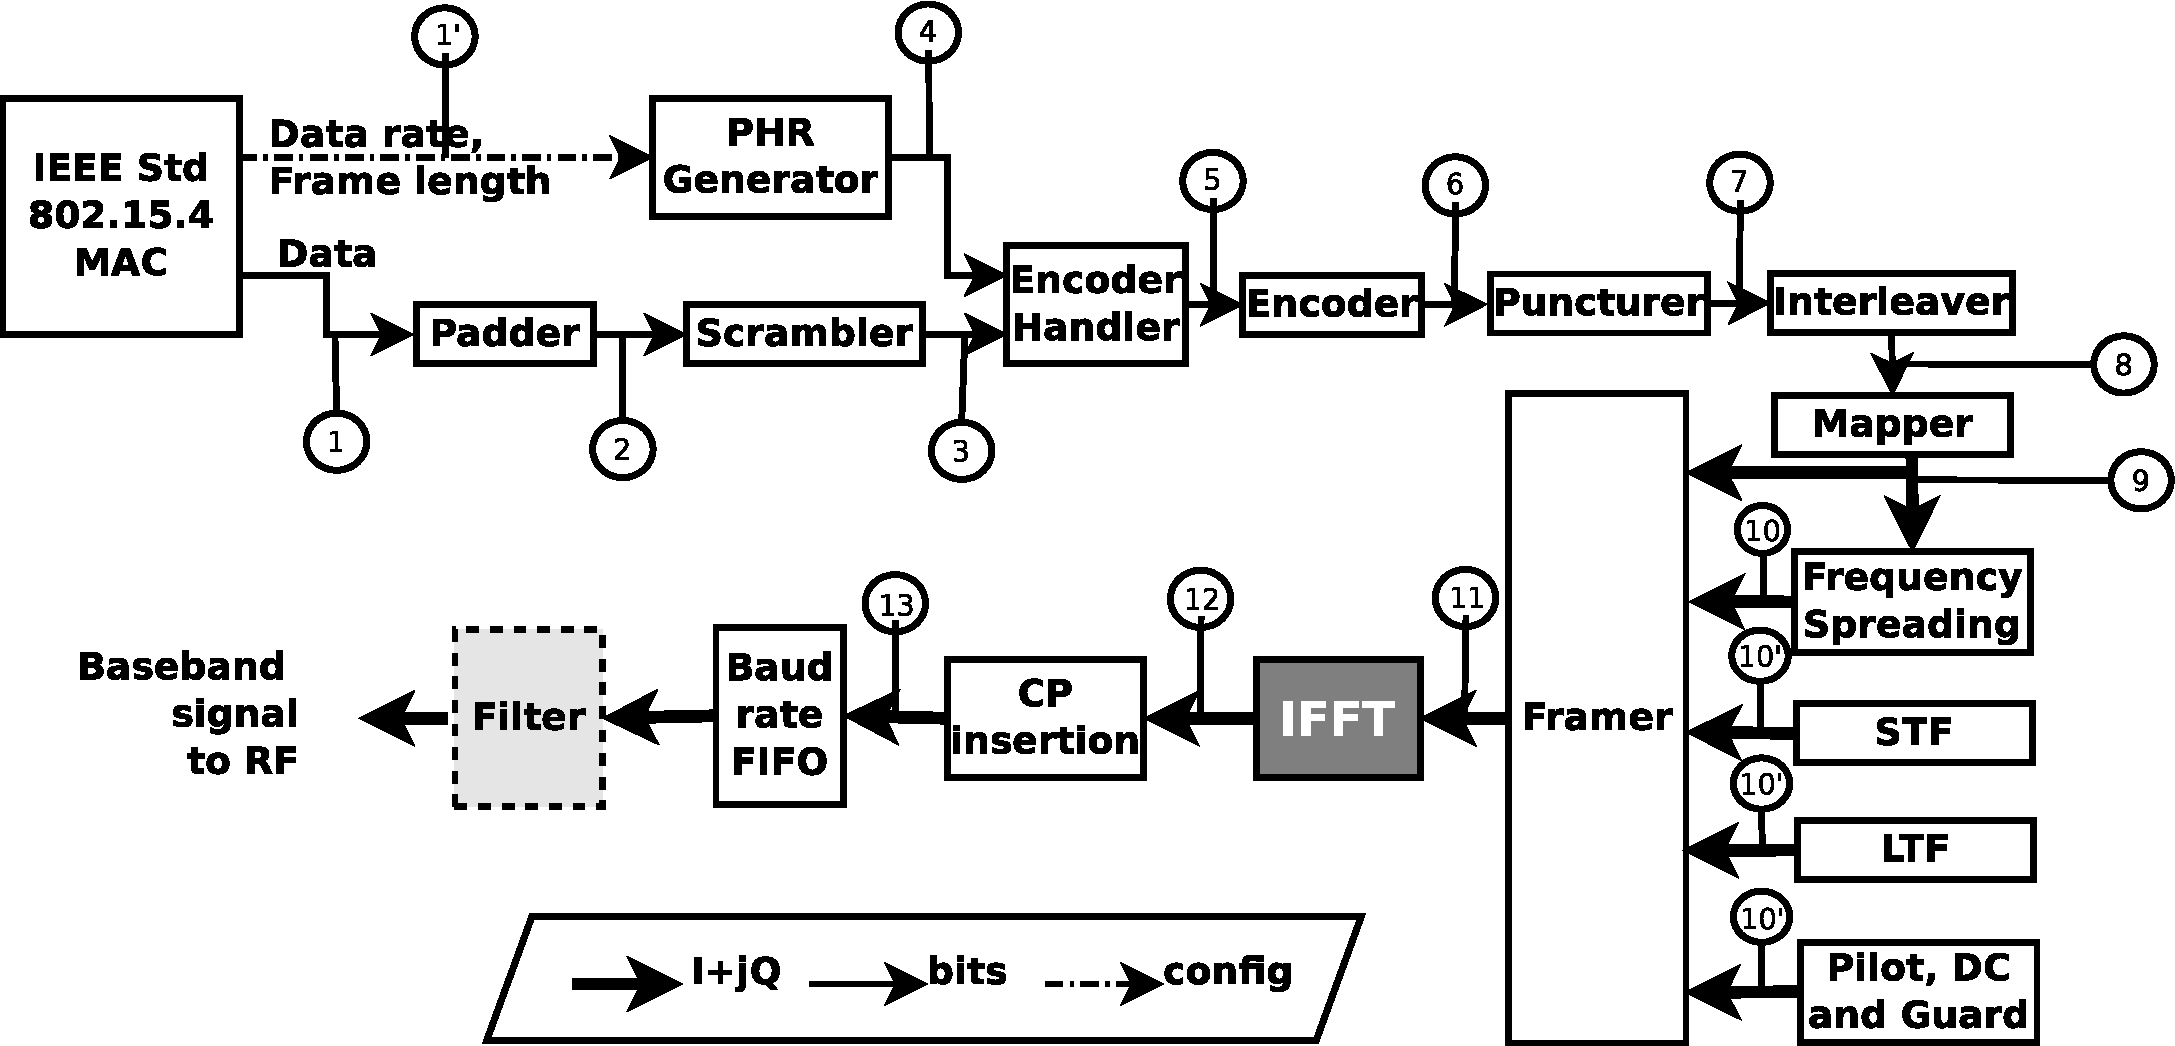
\includegraphics[width=0.9\textwidth]
      {./figures/OFDM_TX_V4_2}
      %{./figures/OFDM_tx_v1}
%     \rule{35em}{0.5pt}
  \caption{MR-OFDM Modulator according to the IEEE802.15.4g Standard}
  \label{fig:ofdm_tx}
\end{figure}


\begin{itemize}
\item \emph{Modulator Data Processing}

\begin{description}
\item [1. ] \emph{PSDU Data}: The payload is received from the upper MAC layer, that is the information that is going to be modulated, i.e. a string of bits that represent some message.
\item [$\boldsymbol{1^{'}}$.] \emph{Configuration}: Generation of Frame length, MCS Level, Data rate, scrambler seed are configurations that come from the MAC layer.  
\item [2. ] \emph{Padder}: PAD bits and TAILS bits are added through the padder block to the PSDU. 
\item [3. ] \emph{Scrambler}: It randomizes the data bits, avoiding long sequences of zeros or ones.
\item [4. ] \emph{PHR Generator}: It generates the PHR according to the configuration chosen in the MAC layer. 
\item [5. ] \emph{Encoder Handler}: Since not all the data is encoded in the same way, this block exchanges between scrambled data and PHR data, in other words, it controls which data to be encoded.  
\item [6. ] \emph{Encoder}: It adds redundancy to the incoming data to add error correction capabilities to the system. 
\item [7 .] \emph{Puncturer}: It changes the data rate according to the MCS. 
\item [8 .] \emph{Interleaver}: Changes the bits order in the data stream. It avoids burst errors.
\item [9 .] \emph{Mapper}: Converts bits to symbols, it maps data bits to a BPSK, QPSK or 16 QAM symbol according to the MCS adopted. 
\end{description}

\item \emph{Modulator Signal Processing}

\begin{description}
\item [10 .] \emph{Frequency Spreader}: Spread the signal in a frequency band greater than the original signal, replicas of the signal are combined to obtain a single symbol.

\item [$\boldsymbol{10'}$ .] \emph{STF}: Short training field, it adds a known sequence to the beginning of the frame, information that is used at the receiver to estimate and correct timing and frequency errors. 

\item [$\boldsymbol{10'}$ .] \emph{LTF}: Long training field. known sequence different from the STF. Although with the same function, used for syncrhonization, frequency error correction and channel equalization at the receiver.

\item [$\boldsymbol{10'}$ .] \emph{Pilot, DC and Guard}: Pilots tones for channel detection and channel gain estimation, DC tone and guard interval to avoid channel interference.  

\item [11 .] \emph{Framer}: The framer rearranges the complex symbols and prepares the OFDM symbol. 

\item [12 .] \emph{Inverse Fourier Transform}: It converts the symbol from frequency domain  to time domain. 

\item [13 .] \emph{CP Insertion}: Adds a Cyclic Prefix, to eliminate inter symbol interference (ISI).

\end{description}

\end{itemize}



% \begin{figure}[hbt]
%   \centering
%     \includegraphics[width=0.9\textwidth]
%       {./figuras/OFDM_DEMO_V_TX_V3}
%       %{./figures/OFDM_tx_v1}
% %     \rule{35em}{0.5pt}
%   \caption{MR-OFDM transmitter according to the IEEE802.15.4g}
%   \label{fig:ofdm_tx}
% \end{figure}

Fig. ~\ref{fig:ofdm_rx} depicts the demodulator structure, its main goal is to   
recover the transmitted data. Basically the receiver undo the process done by the transmitter, however, before this can be accomplished, it has to deal with synchronization issues. Timing synchronization must be attain as well as frequency errors corrected to revert the process done in the transmitter. This is why almost all the signal processing part of the receiver is dedicated to synchronization and frequency error correction. Frequency synchronization and its implementation is one of the topics of this work, specific on the Integer Carrier Frequency Offset (\ac{icfo}) which is estimated and corrected by the block highlighted in Fig.~\ref{fig:ofdm_rx}. A detailed description of the ICFO is found in section~\ref{sec:icfo}. The processing involved at the demodulator is as follows:


\begin{figure}[hbt]
  \centering
    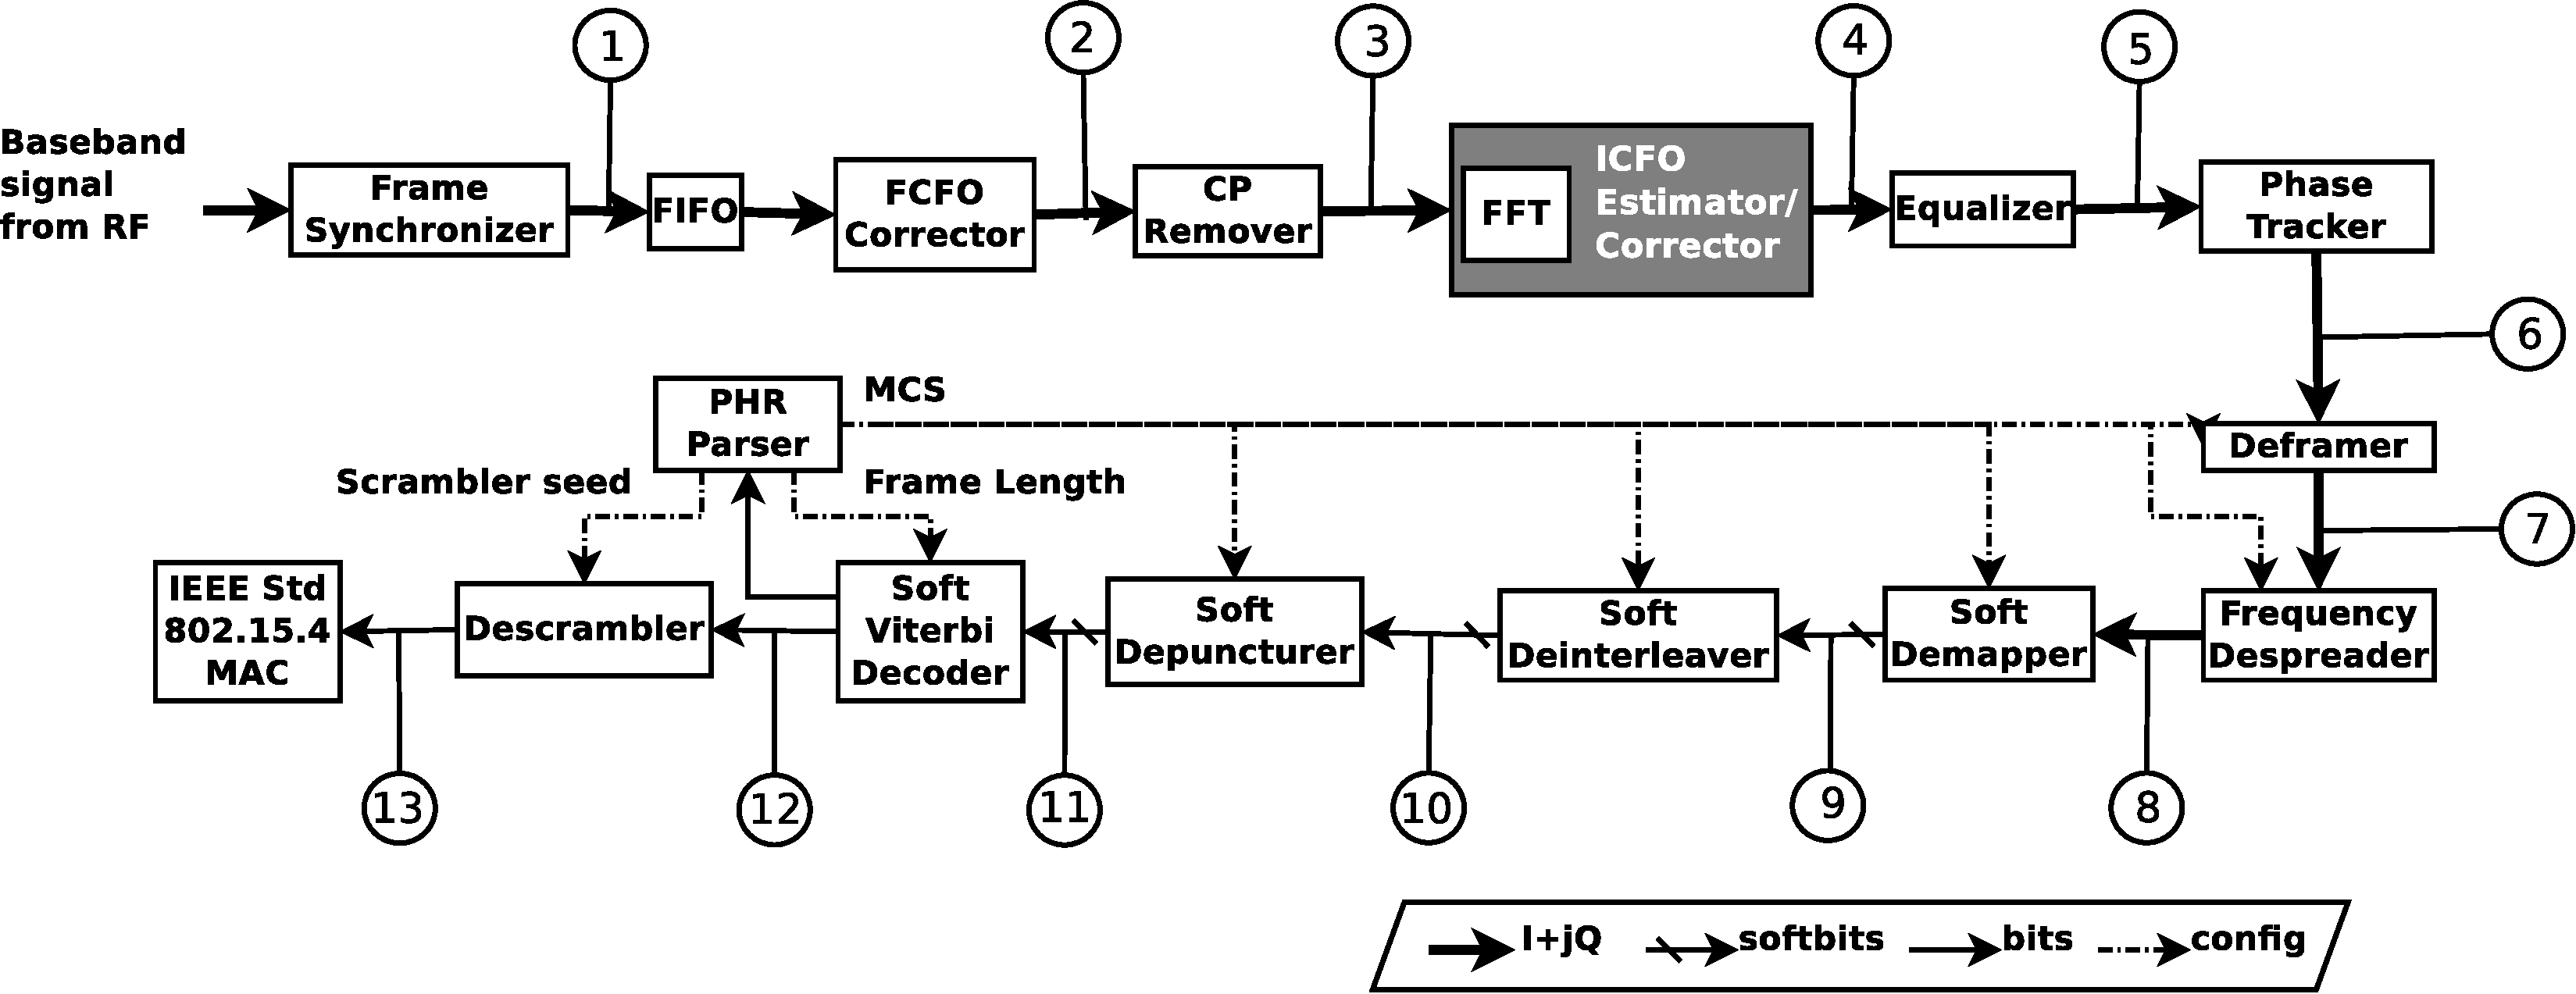
\includegraphics[width=1\textwidth]
      {./figures/OFDM_RX_V7_d}
%     \rule{35ea}{0.5pt}
  \caption{Implemented MR-OFDM receiver}
  \label{fig:ofdm_rx}
\end{figure}

\begin{itemize}
\item \emph{RX Signal Processing}

\begin{description}
%\item [1. ] \emph{Frame Synchronizer} The data at this point is synrhonizer in time, the frame synchronizer find the exact point in which the frame starts. 
\item [1. ] \emph{Frame Synchronizer}: The first step in the OFDM demodulation is the time synchronization. It determines the starting point of the OFDM frame.  
\item [2.] \emph{Fractional CFO}: The frequency error is divided into two parts, a fractional part and a integer part regarding the subcarrier space. In the approach chosen in this work, the fractional correction is performed first. 
\item [3. ] \emph{CP Remover}:  The prepended copy of the symbol end, to combat ISI, is removed.
\item [4. ] \emph{FFT/Integer CFO}: Integer Carrier Frequency Offset estimation/correction is performed and time domain to frequency domain transformation is performed.  
\item [5. ] \emph{Equalizer}: Removing the channel effect over the modulated signal with equalization. 
\item [6. ] \emph{Phase Tracker}: Phase correction for residual errors not corrected in previous stages.    
\item [7. ] \emph{Deframer}: The frame is decomposed into its constituent parts, namely, DC and pilots tones,  Guard intervals, PSDU and PHR.
\item [8 .] \emph{Frequency Despreader}: The frequency spreading is reverted, the replicas in frequency domain are removed. 
\item [9 .] \emph{Soft demaper}: From symbols to bits, from this point only data bits are processed.
\end{description}

\item \emph{RX Data Processing}

\begin{description}
\item [10 .] \emph{Soft deinterleaver}: Rearranges the data in order to revert the process done by the interleaver at the transmitter. 

\item [11 .] \emph{Soft Depuncturer}: Reverts the process of the puncturing at the transmitter. 

\item [12 .] \emph{Viterbi Decoder}: The decoding of the data to perform Forward Error Correction, depending on the noise levels in the transmission the output at this stage is free or with much less errors than before.  

\item [13 .] \emph{Descrambler}: Returns the original data sequence, the payload or PSDU data.  

\end{description}

\end{itemize}

%Implementations for ASIC and prototyping in FPGA of the signal processing parts of TX and RX are to be analyzed and researched for this work. 

This chapter described briefly the MR-OFDM mode of the IEEE802.15.4g standard. The technical aspects covered, and the requirements of this standard, will define the characteristics of the implementations of this work. 

%As can be seen from the specifications the MR-OFDM mode of this standard shows a simple design, although it is the more complex MR mode of the standard. Data rates are low and a low-power and low-area design is intended from this specification. In the following chapters, implementation issues are to be addressed concerning the MR-OFDM, area power and timing will be the main metrics by which implementations are going to be constrained. 
